\section{Measurements}
\label{sec:measurements}

\begin{figure}[tb]
    \centering
    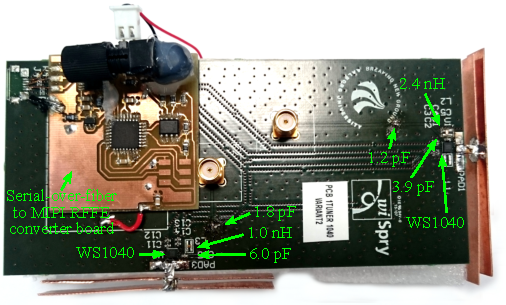
\includegraphics{img/meas/lassedouble}
    \caption{Antenna prototype with MEMS tuners. The converter board converts UART commands from a PC to MIPI RFFE commands, setting the capacitance of the tuners. Component values are annotated.}
    \label{fig:pcb}
\end{figure}

\begin{figure}[tb]
    \centering
    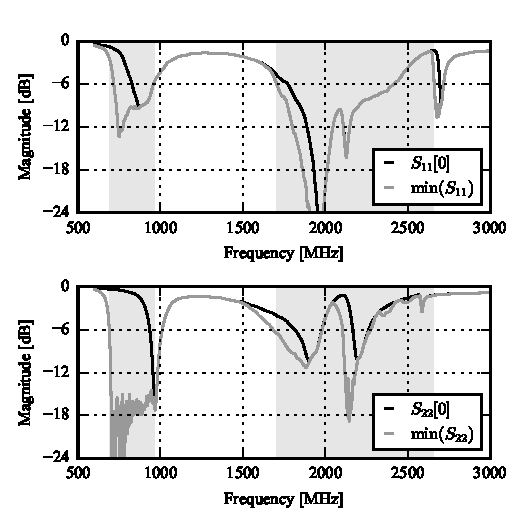
\includegraphics{img/meas/sparams}
    \caption{Measured $S$-parameters for the top and the side antenna when sweeping the tuner from around \SI{0.6}{pF} to \SI{6}{pF} (top antenna) and from around \SI{1.2}{pF} to \SI{12}{pF} (side antenna). Here, $[0]$ marks the minimum capacitance and $\min()$ marks the sweep.}
    \label{fig:meas_sparams}
\end{figure}

The antennas have been built and soldered on to a PCB with a WiSpry WS1040 MEMS tuner for each antenna, as seen in Fig.~\ref{fig:pcb}. Compared to the simplified simulations described in Sec.~\ref{sec:simulations}, the matching at high frequencies appeared troublesome. A shunt capacitor has been soldered onto the transmission lines for each antennas to improve this problem. 
The resulting $S$-parameters are shown in Fig.~\ref{fig:meas_sparams}. It is clear that both antennas cover the low band at \SI{6}{dB} return loss over the tunable range. At the same time, the top antenna covers most of the top band up until \SI{2400}{MHz} while the side antenna lacks bandwidth between \SI{1980}{MHz} and \SI{2110}{MHz} and between \SI{2270}{MHz} and \SI{2650}{MHz}.

\begin{figure}[tb]
    \centering
    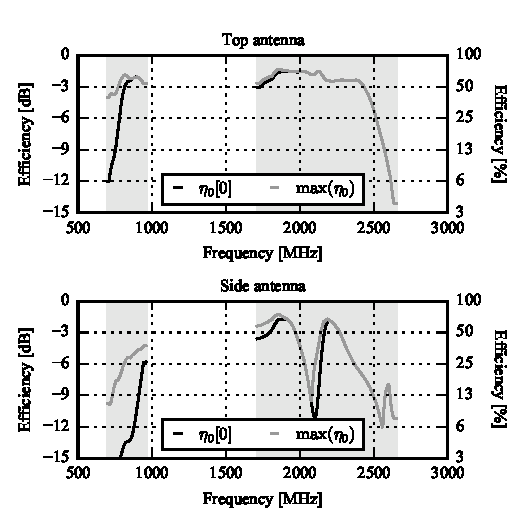
\includegraphics{img/meas/efficiency}
    \caption{Measured total efficiency for the top and the side antenna when sweeping the tuner from around \SI{0.6}{pF} to \SI{6}{pF} (top antenna) and from around \SI{1.2}{pF} to \SI{12}{pF} (side antenna). Here, $[0]$ marks the minimum capacitance and $\max()$ marks the sweep.}
    \label{fig:meas_eff}
\end{figure}

The measured total efficiency when sweeping the tuner is shown in Fig.~\ref{fig:meas_eff}. The top antenna covers all of the low band at around \SI{-3}{dB} efficiency while covering the high band up until \SI{2440}{MHz}. The total efficiency of the side antenna peaks at \SI{-4.1}{dB} in the low band with a minimum at \SI{-9.9}{dB}. The high band is covered from \SI{1710}{MHz} to \SI{1925}{MHz} and from \SI{2095}{MHz} to \SI{2230}{MHz} over its tunable range.

